% Options for packages loaded elsewhere
% Options for packages loaded elsewhere
\PassOptionsToPackage{unicode}{hyperref}
\PassOptionsToPackage{hyphens}{url}
\PassOptionsToPackage{dvipsnames,svgnames,x11names}{xcolor}
%
\documentclass[
  letterpaper,
  DIV=11,
  numbers=noendperiod]{scrartcl}
\usepackage{xcolor}
\usepackage[top=10mm,bottom=10mm,left=15mm,right=15mm]{geometry}
\usepackage{amsmath,amssymb}
\setcounter{secnumdepth}{-\maxdimen} % remove section numbering
\usepackage{iftex}
\ifPDFTeX
  \usepackage[T1]{fontenc}
  \usepackage[utf8]{inputenc}
  \usepackage{textcomp} % provide euro and other symbols
\else % if luatex or xetex
  \usepackage{unicode-math} % this also loads fontspec
  \defaultfontfeatures{Scale=MatchLowercase}
  \defaultfontfeatures[\rmfamily]{Ligatures=TeX,Scale=1}
\fi
\usepackage{lmodern}
\ifPDFTeX\else
  % xetex/luatex font selection
\fi
% Use upquote if available, for straight quotes in verbatim environments
\IfFileExists{upquote.sty}{\usepackage{upquote}}{}
\IfFileExists{microtype.sty}{% use microtype if available
  \usepackage[]{microtype}
  \UseMicrotypeSet[protrusion]{basicmath} % disable protrusion for tt fonts
}{}
\makeatletter
\@ifundefined{KOMAClassName}{% if non-KOMA class
  \IfFileExists{parskip.sty}{%
    \usepackage{parskip}
  }{% else
    \setlength{\parindent}{0pt}
    \setlength{\parskip}{6pt plus 2pt minus 1pt}}
}{% if KOMA class
  \KOMAoptions{parskip=half}}
\makeatother
% Make \paragraph and \subparagraph free-standing
\makeatletter
\ifx\paragraph\undefined\else
  \let\oldparagraph\paragraph
  \renewcommand{\paragraph}{
    \@ifstar
      \xxxParagraphStar
      \xxxParagraphNoStar
  }
  \newcommand{\xxxParagraphStar}[1]{\oldparagraph*{#1}\mbox{}}
  \newcommand{\xxxParagraphNoStar}[1]{\oldparagraph{#1}\mbox{}}
\fi
\ifx\subparagraph\undefined\else
  \let\oldsubparagraph\subparagraph
  \renewcommand{\subparagraph}{
    \@ifstar
      \xxxSubParagraphStar
      \xxxSubParagraphNoStar
  }
  \newcommand{\xxxSubParagraphStar}[1]{\oldsubparagraph*{#1}\mbox{}}
  \newcommand{\xxxSubParagraphNoStar}[1]{\oldsubparagraph{#1}\mbox{}}
\fi
\makeatother


\usepackage{longtable,booktabs,array}
\newcounter{none} % for unnumbered tables
\usepackage{calc} % for calculating minipage widths
% Correct order of tables after \paragraph or \subparagraph
\usepackage{etoolbox}
\makeatletter
\patchcmd\longtable{\par}{\if@noskipsec\mbox{}\fi\par}{}{}
\makeatother
% Allow footnotes in longtable head/foot
\IfFileExists{footnotehyper.sty}{\usepackage{footnotehyper}}{\usepackage{footnote}}
\makesavenoteenv{longtable}
\usepackage{graphicx}
\makeatletter
\newsavebox\pandoc@box
\newcommand*\pandocbounded[1]{% scales image to fit in text height/width
  \sbox\pandoc@box{#1}%
  \Gscale@div\@tempa{\textheight}{\dimexpr\ht\pandoc@box+\dp\pandoc@box\relax}%
  \Gscale@div\@tempb{\linewidth}{\wd\pandoc@box}%
  \ifdim\@tempb\p@<\@tempa\p@\let\@tempa\@tempb\fi% select the smaller of both
  \ifdim\@tempa\p@<\p@\scalebox{\@tempa}{\usebox\pandoc@box}%
  \else\usebox{\pandoc@box}%
  \fi%
}
% Set default figure placement to htbp
\def\fps@figure{htbp}
\makeatother





\setlength{\emergencystretch}{3em} % prevent overfull lines

\providecommand{\tightlist}{%
  \setlength{\itemsep}{0pt}\setlength{\parskip}{0pt}}



 


\usepackage{array}
\providecommand{\huxb}[2]{\arrayrulecolor[RGB]{#1}\global\arrayrulewidth=#2pt}
\providecommand{\huxvb}[2]{\color[RGB]{#1}\vrule width #2pt}
\providecommand{\huxtpad}[1]{\rule{0pt}{#1}}
\providecommand{\huxbpad}[1]{\rule[-#1]{0pt}{#1}}
\usepackage{caption}
\usepackage{graphicx}
\usepackage{siunitx}
\usepackage[normalem]{ulem}
\usepackage{colortbl}
\usepackage{multirow}
\usepackage{hhline}
\usepackage{calc}
\usepackage{tabularx}
\usepackage{longtable}
\usepackage{threeparttable}
\usepackage{threeparttablex}
\usepackage{wrapfig}
\usepackage{adjustbox}
\usepackage{hyperref}
\KOMAoption{captions}{tableheading,figureheading}
\makeatletter
\@ifpackageloaded{caption}{}{\usepackage{caption}}
\AtBeginDocument{%
\ifdefined\contentsname
  \renewcommand*\contentsname{Table of contents}
\else
  \newcommand\contentsname{Table of contents}
\fi
\ifdefined\listfigurename
  \renewcommand*\listfigurename{List of Figures}
\else
  \newcommand\listfigurename{List of Figures}
\fi
\ifdefined\listtablename
  \renewcommand*\listtablename{List of Tables}
\else
  \newcommand\listtablename{List of Tables}
\fi
\ifdefined\figurename
  \renewcommand*\figurename{Figure}
\else
  \newcommand\figurename{Figure}
\fi
\ifdefined\tablename
  \renewcommand*\tablename{Table}
\else
  \newcommand\tablename{Table}
\fi
}
\@ifpackageloaded{float}{}{\usepackage{float}}
\floatstyle{ruled}
\@ifundefined{c@chapter}{\newfloat{codelisting}{h}{lop}}{\newfloat{codelisting}{h}{lop}[chapter]}
\floatname{codelisting}{Listing}
\newcommand*\listoflistings{\listof{codelisting}{List of Listings}}
\makeatother
\makeatletter
\makeatother
\makeatletter
\@ifpackageloaded{caption}{}{\usepackage{caption}}
\@ifpackageloaded{subcaption}{}{\usepackage{subcaption}}
\makeatother
\usepackage{bookmark}
\IfFileExists{xurl.sty}{\usepackage{xurl}}{} % add URL line breaks if available
\urlstyle{same}
% fallback for those not using the hyperref driver hyperxmp:
\makeatletter
\@ifundefined{xmpquote}{\newcommand{\xmpquote}[1]{#1}}{}
\makeatother
\hypersetup{
  pdftitle={Measurement: Homework 2},
  pdfauthor={Beltrán González Luis Enrique},
  colorlinks=true,
  linkcolor={blue},
  filecolor={Maroon},
  citecolor={Blue},
  urlcolor={Blue},
  pdfcreator={LaTeX via pandoc}}


\title{Measurement: Homework 2}
\author{Beltrán González Luis Enrique}
\date{2026-10-09}
\begin{document}
\maketitle


\section{1 Child Mortality in Côte d'Ivoire (6
points)}\label{child-mortality-in-cuxf4te-divoire-6-points}

\subsection{1. Sampling (1 points)}\label{sampling-1-points}

\textbf{(a) How should you transform pweight to obtain a weight that
allows you to estimate statistics on the population of women in Cote
d'Ivoire? Explain your computations.}

I can use the pweight column to balance the class distribution of the
sample to match the population distribution. The \texttt{pweight} column
contains sample weights that modify the contribution of each observation
to the overall statistics. It works as a frequency multiplier, where
each observation is counted as if it were \texttt{pweight} number of
observations. In practice, R can use the pweight column to compute
weighted statistics, such as means and proportions by using the
\texttt{weights} argument in functions like \texttt{lm()} or
\texttt{survey::svydesign()}. Internally, weighted functions such as
weighted means and lm will multiply each observation by its
corresponding weight. For example a weighted mean will be computed using
equation Equation~\ref{eq-weighted_mean}, and weighted linear regression
will minimize the weighted sum of squared residuals, as shown in
equation Equation~\ref{eq-weighted_lm}.

\begin{equation}\protect\phantomsection\label{eq-weighted_mean}{
\bar{x}_w = \frac{\sum_{i=1}^{n} w_i x_i}{\sum_{i=1}^{n} w_i}
}\end{equation}

\begin{equation}\protect\phantomsection\label{eq-weighted_lm}{
\sum_{i=1}^{n} w_i (y_i - \hat{y}_i)^2
}\end{equation}

\subsection{2. Measurement of under 5 mortality rate (5
points)}\label{measurement-of-under-5-mortality-rate-5-points}

\textbf{(a) What method can be deemed preferable and why? Give the pros
and cons of both methods.}

The preferable method is method 2 (M2) because method 1 (M1)
underestimates the mortality rate by not capturing the deaths that occur
after the survey period. Figure~\ref{fig-mortality} shows graphycally
the surveyed groups: the x-axis represents the age of the child at the
time of the survey, and the y-axis represents the age of the child at
the time of death. The red arrow at 45 degrees indicates the frontier of
possible outcomes, since by definition noone can die after their current
age, the survey caputures outcomes below the frontier. Notice M1
captures area B and drops area C underestimating the true mortality
rate. M2 captures area C which represents the true mortality rate. For
example a surveyed mother has a child one year before the survey and the
child dies the year after the survey (area C in
Figure~\ref{fig-mortality}), M1 will not capture his death because by
definition nothing can die after its current age.

M1

\begin{itemize}
\tightlist
\item
  Pros: it is easy to compute, captures the most recent deaths
  (recency).
\item
  Cons: underestimates the mortality rate, downward biased, does not
  capture deaths after the survey period.
\end{itemize}

M2

\begin{itemize}
\tightlist
\item
  Pros: provides a robust estimate of the true mortality rate.
\item
  Cons: it requires a longer period of time to capture deaths, less
  recent than M1.
\end{itemize}

\begin{figure}

\caption{\label{fig-mortality}Mortality estimator analysis}

\centering{

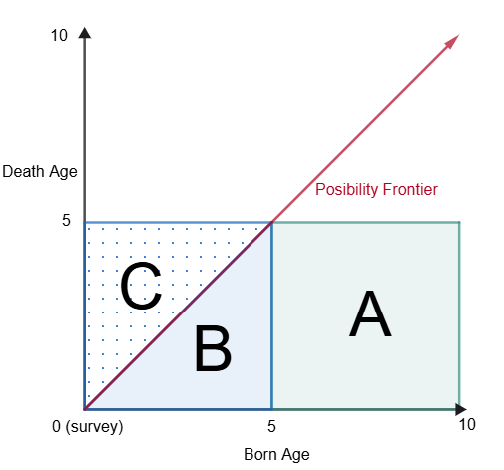
\includegraphics[width=0.5\linewidth,height=\textheight,keepaspectratio]{img/mortality_chart.png}

}

\end{figure}%

\textbf{(b) Child mortality rates in Côte d'Ivoire.}

\textbf{i. Compute mortality rates with both methods for boys and girls
separately (don't forget the weights).}

 
\begin{table}[ht]
\begin{centerbox}
\begin{threeparttable}
\captionsetup{justification=centering,singlelinecheck=off}
\caption{Child mortality rates in Côte d'Ivoire, by sex and method.}
 \label{tbl-child_mortality}\setlength{\tabcolsep}{0pt}
\begin{tabular}{l l l l l l l l}


\hhline{>{\huxb{0, 0, 0}{0.8}}->{\huxb{0, 0, 0}{0.8}}->{\huxb{0, 0, 0}{0.8}}->{\huxb{0, 0, 0}{0.8}}->{\huxb{0, 0, 0}{0.8}}->{\huxb{0, 0, 0}{0.8}}->{\huxb{0, 0, 0}{0.8}}->{\huxb{0, 0, 0}{0.8}}-}
\arrayrulecolor{black}

\multicolumn{1}{!{\huxvb{0, 0, 0}{0}}c!{\huxvb{0, 0, 0}{0}}}{\huxtpad{1.5pt + 1em}\centering \hspace{1.5pt}  \hspace{1.5pt}\huxbpad{1.5pt}} &
\multicolumn{1}{c!{\huxvb{0, 0, 0}{0}}}{\huxtpad{1.5pt + 1em}\centering \hspace{1.5pt} M1 (Boys) \hspace{1.5pt}\huxbpad{1.5pt}} &
\multicolumn{1}{c!{\huxvb{0, 0, 0}{0}}}{\huxtpad{1.5pt + 1em}\centering \hspace{1.5pt} M2 (Boys) \hspace{1.5pt}\huxbpad{1.5pt}} &
\multicolumn{1}{c!{\huxvb{0, 0, 0}{0}}}{\huxtpad{1.5pt + 1em}\centering \hspace{1.5pt} Diff (Boys) \hspace{1.5pt}\huxbpad{1.5pt}} &
\multicolumn{1}{c!{\huxvb{0, 0, 0}{0}}}{\huxtpad{1.5pt + 1em}\centering \hspace{1.5pt} M1 (Girls) \hspace{1.5pt}\huxbpad{1.5pt}} &
\multicolumn{1}{c!{\huxvb{0, 0, 0}{0}}}{\huxtpad{1.5pt + 1em}\centering \hspace{1.5pt} M2 (Girls) \hspace{1.5pt}\huxbpad{1.5pt}} &
\multicolumn{1}{c!{\huxvb{0, 0, 0}{0}}}{\huxtpad{1.5pt + 1em}\centering \hspace{1.5pt} Diff (Girls) \hspace{1.5pt}\huxbpad{1.5pt}} &
\multicolumn{1}{c!{\huxvb{0, 0, 0}{0}}}{\huxtpad{1.5pt + 1em}\centering \hspace{1.5pt} Diff M2 G-B \hspace{1.5pt}\huxbpad{1.5pt}} \tabularnewline[-0.5pt]


\hhline{>{\huxb{255, 255, 255}{0.4}}->{\huxb{0, 0, 0}{0.4}}->{\huxb{0, 0, 0}{0.4}}->{\huxb{0, 0, 0}{0.4}}->{\huxb{0, 0, 0}{0.4}}->{\huxb{0, 0, 0}{0.4}}->{\huxb{0, 0, 0}{0.4}}->{\huxb{0, 0, 0}{0.4}}-}
\arrayrulecolor{black}

\multicolumn{1}{!{\huxvb{0, 0, 0}{0}}l!{\huxvb{0, 0, 0}{0}}}{\huxtpad{1.5pt + 1em}\raggedright \hspace{1.5pt} Mortality rate \hspace{1.5pt}\huxbpad{1.5pt}} &
\multicolumn{1}{r!{\huxvb{0, 0, 0}{0}}}{\huxtpad{1.5pt + 1em}\raggedleft \hspace{1.5pt} 0.117 *** \hspace{1.5pt}\huxbpad{1.5pt}} &
\multicolumn{1}{r!{\huxvb{0, 0, 0}{0}}}{\huxtpad{1.5pt + 1em}\raggedleft \hspace{1.5pt} 0.135 *** \hspace{1.5pt}\huxbpad{1.5pt}} &
\multicolumn{1}{r!{\huxvb{0, 0, 0}{0}}}{\huxtpad{1.5pt + 1em}\raggedleft \hspace{1.5pt} 0.017 \hspace{1.5pt}\huxbpad{1.5pt}} &
\multicolumn{1}{r!{\huxvb{0, 0, 0}{0}}}{\huxtpad{1.5pt + 1em}\raggedleft \hspace{1.5pt} 0.084 *** \hspace{1.5pt}\huxbpad{1.5pt}} &
\multicolumn{1}{r!{\huxvb{0, 0, 0}{0}}}{\huxtpad{1.5pt + 1em}\raggedleft \hspace{1.5pt} 0.115 *** \hspace{1.5pt}\huxbpad{1.5pt}} &
\multicolumn{1}{r!{\huxvb{0, 0, 0}{0}}}{\huxtpad{1.5pt + 1em}\raggedleft \hspace{1.5pt} 0.031 *** \hspace{1.5pt}\huxbpad{1.5pt}} &
\multicolumn{1}{r!{\huxvb{0, 0, 0}{0}}}{\huxtpad{1.5pt + 1em}\raggedleft \hspace{1.5pt} -0.020 * \hspace{1.5pt}\huxbpad{1.5pt}} \tabularnewline[-0.5pt]


\hhline{}
\arrayrulecolor{black}

\multicolumn{1}{!{\huxvb{0, 0, 0}{0}}l!{\huxvb{0, 0, 0}{0}}}{\huxtpad{1.5pt + 1em}\raggedright \hspace{1.5pt}  \hspace{1.5pt}\huxbpad{1.5pt}} &
\multicolumn{1}{r!{\huxvb{0, 0, 0}{0}}}{\huxtpad{1.5pt + 1em}\raggedleft \hspace{1.5pt} (0.007) \hspace{1.5pt}\huxbpad{1.5pt}} &
\multicolumn{1}{r!{\huxvb{0, 0, 0}{0}}}{\huxtpad{1.5pt + 1em}\raggedleft \hspace{1.5pt} (0.008) \hspace{1.5pt}\huxbpad{1.5pt}} &
\multicolumn{1}{r!{\huxvb{0, 0, 0}{0}}}{\huxtpad{1.5pt + 1em}\raggedleft \hspace{1.5pt} (0.011) \hspace{1.5pt}\huxbpad{1.5pt}} &
\multicolumn{1}{r!{\huxvb{0, 0, 0}{0}}}{\huxtpad{1.5pt + 1em}\raggedleft \hspace{1.5pt} (0.007) \hspace{1.5pt}\huxbpad{1.5pt}} &
\multicolumn{1}{r!{\huxvb{0, 0, 0}{0}}}{\huxtpad{1.5pt + 1em}\raggedleft \hspace{1.5pt} (0.008) \hspace{1.5pt}\huxbpad{1.5pt}} &
\multicolumn{1}{r!{\huxvb{0, 0, 0}{0}}}{\huxtpad{1.5pt + 1em}\raggedleft \hspace{1.5pt} (0.010) \hspace{1.5pt}\huxbpad{1.5pt}} &
\multicolumn{1}{r!{\huxvb{0, 0, 0}{0}}}{\huxtpad{1.5pt + 1em}\raggedleft \hspace{1.5pt} (0.011) \hspace{1.5pt}\huxbpad{1.5pt}} \tabularnewline[-0.5pt]


\hhline{>{\huxb{255, 255, 255}{0.4}}->{\huxb{0, 0, 0}{0.4}}->{\huxb{0, 0, 0}{0.4}}->{\huxb{0, 0, 0}{0.4}}->{\huxb{0, 0, 0}{0.4}}->{\huxb{0, 0, 0}{0.4}}->{\huxb{0, 0, 0}{0.4}}->{\huxb{0, 0, 0}{0.4}}-}
\arrayrulecolor{black}

\multicolumn{1}{!{\huxvb{0, 0, 0}{0}}l!{\huxvb{0, 0, 0}{0}}}{\huxtpad{1.5pt + 1em}\raggedright \hspace{1.5pt} N \hspace{1.5pt}\huxbpad{1.5pt}} &
\multicolumn{1}{r!{\huxvb{0, 0, 0}{0}}}{\huxtpad{1.5pt + 1em}\raggedleft \hspace{1.5pt} 1431 \hspace{1.5pt}\huxbpad{1.5pt}} &
\multicolumn{1}{r!{\huxvb{0, 0, 0}{0}}}{\huxtpad{1.5pt + 1em}\raggedleft \hspace{1.5pt} 1332 \hspace{1.5pt}\huxbpad{1.5pt}} &
\multicolumn{1}{r!{\huxvb{0, 0, 0}{0}}}{\huxtpad{1.5pt + 1em}\raggedleft \hspace{1.5pt}  \hspace{1.5pt}\huxbpad{1.5pt}} &
\multicolumn{1}{r!{\huxvb{0, 0, 0}{0}}}{\huxtpad{1.5pt + 1em}\raggedleft \hspace{1.5pt} 1428 \hspace{1.5pt}\huxbpad{1.5pt}} &
\multicolumn{1}{r!{\huxvb{0, 0, 0}{0}}}{\huxtpad{1.5pt + 1em}\raggedleft \hspace{1.5pt} 1291 \hspace{1.5pt}\huxbpad{1.5pt}} &
\multicolumn{1}{r!{\huxvb{0, 0, 0}{0}}}{\huxtpad{1.5pt + 1em}\raggedleft \hspace{1.5pt}  \hspace{1.5pt}\huxbpad{1.5pt}} &
\multicolumn{1}{r!{\huxvb{0, 0, 0}{0}}}{\huxtpad{1.5pt + 1em}\raggedleft \hspace{1.5pt}  \hspace{1.5pt}\huxbpad{1.5pt}} \tabularnewline[-0.5pt]


\hhline{}
\arrayrulecolor{black}

\multicolumn{1}{!{\huxvb{0, 0, 0}{0}}l!{\huxvb{0, 0, 0}{0}}}{\huxtpad{1.5pt + 1em}\raggedright \hspace{1.5pt} R2 \hspace{1.5pt}\huxbpad{1.5pt}} &
\multicolumn{1}{r!{\huxvb{0, 0, 0}{0}}}{\huxtpad{1.5pt + 1em}\raggedleft \hspace{1.5pt} 0.000 \hspace{1.5pt}\huxbpad{1.5pt}} &
\multicolumn{1}{r!{\huxvb{0, 0, 0}{0}}}{\huxtpad{1.5pt + 1em}\raggedleft \hspace{1.5pt} 0.000 \hspace{1.5pt}\huxbpad{1.5pt}} &
\multicolumn{1}{r!{\huxvb{0, 0, 0}{0}}}{\huxtpad{1.5pt + 1em}\raggedleft \hspace{1.5pt}  \hspace{1.5pt}\huxbpad{1.5pt}} &
\multicolumn{1}{r!{\huxvb{0, 0, 0}{0}}}{\huxtpad{1.5pt + 1em}\raggedleft \hspace{1.5pt} 0.000 \hspace{1.5pt}\huxbpad{1.5pt}} &
\multicolumn{1}{r!{\huxvb{0, 0, 0}{0}}}{\huxtpad{1.5pt + 1em}\raggedleft \hspace{1.5pt} 0.000 \hspace{1.5pt}\huxbpad{1.5pt}} &
\multicolumn{1}{r!{\huxvb{0, 0, 0}{0}}}{\huxtpad{1.5pt + 1em}\raggedleft \hspace{1.5pt}  \hspace{1.5pt}\huxbpad{1.5pt}} &
\multicolumn{1}{r!{\huxvb{0, 0, 0}{0}}}{\huxtpad{1.5pt + 1em}\raggedleft \hspace{1.5pt}  \hspace{1.5pt}\huxbpad{1.5pt}} \tabularnewline[-0.5pt]


\hhline{>{\huxb{0, 0, 0}{0.8}}->{\huxb{0, 0, 0}{0.8}}->{\huxb{0, 0, 0}{0.8}}->{\huxb{0, 0, 0}{0.8}}->{\huxb{0, 0, 0}{0.8}}->{\huxb{0, 0, 0}{0.8}}->{\huxb{0, 0, 0}{0.8}}->{\huxb{0, 0, 0}{0.8}}-}
\arrayrulecolor{black}
\end{tabular}
\begin{tablenotes}[flushleft]
\item[] Significance: *** p $<$ 0.01; ** p $<$ 0.05; * p $<$ 0.1
\end{tablenotes}
\end{threeparttable}\par\end{centerbox}

\end{table}
 

\textbf{ii. Compare and comment.}

Table \ref{tbl-child_mortality} shows the estimated child mortality
rates in Côte d'Ivoire for boys and girls using both methods and their
differences. The results confirm our theory of M1 underestimating the
true mortality rate. We can clearly see the method estimates differences
are positive indicating that M1 systematically underestimates the true
mortality rate estimated by M2. Using the best method (M2), the average
mortality rate for boys is 13.5\% and for girls is 11.9\%. The
difference between girls and boys is -2 percentage points and
statitically significant at the 90\% confidence level, indicating that
boys have a higher mortality rate than girls.

\section{2 Health status, nutritional status and wealth in Côte d'Ivoire
(7
points)}\label{health-status-nutritional-status-and-wealth-in-cuxf4te-divoire-7-points}

\emph{Stunted children are defined as children showing a height stature
that is lower than the median of the reference population by 2 standard
deviations measured on the same reference population. That is children
such as the z-score is lower than -2 (}\(z \le -2\)), where the z-score
is given by the following formula:

\[Z = \frac{\text{height} - \text{WHOMedian}(\text{sex}, \text{age})}{\text{WHOstdev}(\text{sex}, \text{age})}\]

\subsection{1. Weight Unit Correction}\label{weight-unit-correction}

\emph{In 2008, the weight could be measured in either kilograms or
hectograms. However, the unit was not systematically reported. It was
therefore assumed that all the weights were reported in kilograms.}

\textbf{(a) Derive an expression for the sample mean weight in this
context, and show that, if we knew just one parameter, we could obtain a
non-biased estimate of the mean weight despite the hectogram issue. (.5
point)}

Let's denote the estimated mean weight as \(W_{\text{obs}}\), the true
mean weight as \(W_{\text{true}}\), and the proportion of weights
measured in hectograms as \(p_h\). The observed mean weight can be
expressed as the sum of the mean weights measured in kg and in
hectograms multiplied by their corresponding probabilities:

\[
\begin{aligned}
E[W_{\text{obs}}] &= (1 - p_h) \cdot W_{\text{true}} + p_h \cdot W_{\text{true}}\cdot 10\\
  &= W_{\text{true}} \cdot (1 - p_h + 10 p_h)\\
  &= W_{\text{true}} \cdot (1 + 9 p_h)
\end{aligned}
\]

Thus, having an estimate of \(p_h\) would allow us to correct the
observed mean weight. Notice that if \(p_h = 0\), then
\(E[W_{\text{obs}}] = W_{\text{true}}\), and if \(p_h = 1\), then
\(E[W_{\text{obs}}] = 10 W_{\text{true}}\).

\textbf{(b) Come up with an empirical criterion to identify hectogram
mistakes, and a graphical way to show the 2008 weight distribution,
before and after correcting for mistakes, compared with the 1988 and
1993 weight distributions. (1 point)}

By looking at the original distribution the weight measurements in 2008
show a wider distribution than the 1988 and 1993 distributions. The 2008
distribution shows a principal component at around 12kg but also shows
multiple peaks at weight \textgreater{} 25kg while the 1988 and 1993
distributions show a principal component at around 12kg with minimal
outliers e.g.~a few values below 1kg. See Figure \ref{fig-distributions}
LHS.

After updating the 2008 weight distribution by dividing all weights
\textgreater{} 25kg by 10, the distribution shows no peaks after 25kg.
See Figure \ref{fig-distributions} RHS.

\begin{figure}

\caption{\label{fig-distributions}Distribution of Weight (kg) Before and
After Correction}

\centering{

\pandocbounded{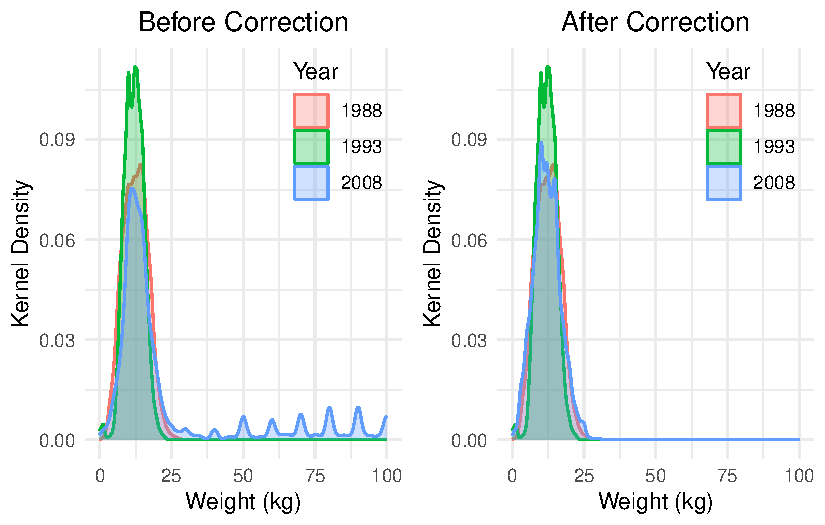
\includegraphics[keepaspectratio]{hw2_files/figure-pdf/fig-distributions-1.pdf}}

}

\end{figure}%

\subsection{2. Z-Score Computation}\label{z-score-computation}

\textbf{Using the variables medheight and stdheight, compute each
child's z-score. (.5 point)} Estimated z-scores are computed using the
mentioned formula. The resulting distribution of z-scores for 2-4 years
old children by year and region is shown in Figure
\ref{fig-distributions_stunted}

\subsection{3. Height Stature over time and across regions (3
points)}\label{height-stature-over-time-and-across-regions-3-points}

\textbf{(a) Estimate the stunting rate for 2-4 years old children over
time in the North, in the South, and at the national level. Decide what
are outliers, and show results both including and excluding outliers.
Comment your results, making all relevant comparisons.}

 
\begin{table}[ht]
\begin{centerbox}
\begin{threeparttable}
\captionsetup{justification=centering,singlelinecheck=off}
\caption{National, North, and South stunting rates for 2-4 years old children including outliers.}
 \label{tbl-stunted_w_outliers}\setlength{\tabcolsep}{0pt}
\begin{tabular}{l l l l l}


\hhline{>{\huxb{0, 0, 0}{0.8}}->{\huxb{0, 0, 0}{0.8}}->{\huxb{0, 0, 0}{0.8}}->{\huxb{0, 0, 0}{0.8}}->{\huxb{0, 0, 0}{0.8}}-}
\arrayrulecolor{black}

\multicolumn{1}{!{\huxvb{0, 0, 0}{0}}c!{\huxvb{0, 0, 0}{0}}}{\huxtpad{1.5pt + 1em}\centering \hspace{1.5pt}  \hspace{1.5pt}\huxbpad{1.5pt}} &
\multicolumn{1}{c!{\huxvb{0, 0, 0}{0}}}{\huxtpad{1.5pt + 1em}\centering \hspace{1.5pt} National \hspace{1.5pt}\huxbpad{1.5pt}} &
\multicolumn{1}{c!{\huxvb{0, 0, 0}{0}}}{\huxtpad{1.5pt + 1em}\centering \hspace{1.5pt} North \hspace{1.5pt}\huxbpad{1.5pt}} &
\multicolumn{1}{c!{\huxvb{0, 0, 0}{0}}}{\huxtpad{1.5pt + 1em}\centering \hspace{1.5pt} South \hspace{1.5pt}\huxbpad{1.5pt}} &
\multicolumn{1}{c!{\huxvb{0, 0, 0}{0}}}{\huxtpad{1.5pt + 1em}\centering \hspace{1.5pt} Diff (North-South) \hspace{1.5pt}\huxbpad{1.5pt}} \tabularnewline[-0.5pt]


\hhline{>{\huxb{255, 255, 255}{0.4}}->{\huxb{0, 0, 0}{0.4}}->{\huxb{0, 0, 0}{0.4}}->{\huxb{0, 0, 0}{0.4}}->{\huxb{0, 0, 0}{0.4}}-}
\arrayrulecolor{black}

\multicolumn{1}{!{\huxvb{0, 0, 0}{0}}l!{\huxvb{0, 0, 0}{0}}}{\huxtpad{1.5pt + 1em}\raggedright \hspace{1.5pt} Year 1988 \hspace{1.5pt}\huxbpad{1.5pt}} &
\multicolumn{1}{r!{\huxvb{0, 0, 0}{0}}}{\huxtpad{1.5pt + 1em}\raggedleft \hspace{1.5pt} 0.263 *** \hspace{1.5pt}\huxbpad{1.5pt}} &
\multicolumn{1}{r!{\huxvb{0, 0, 0}{0}}}{\huxtpad{1.5pt + 1em}\raggedleft \hspace{1.5pt} 0.307 *** \hspace{1.5pt}\huxbpad{1.5pt}} &
\multicolumn{1}{r!{\huxvb{0, 0, 0}{0}}}{\huxtpad{1.5pt + 1em}\raggedleft \hspace{1.5pt} 0.247 *** \hspace{1.5pt}\huxbpad{1.5pt}} &
\multicolumn{1}{r!{\huxvb{0, 0, 0}{0}}}{\huxtpad{1.5pt + 1em}\raggedleft \hspace{1.5pt} 0.060 ** \hspace{1.5pt}\huxbpad{1.5pt}} \tabularnewline[-0.5pt]


\hhline{}
\arrayrulecolor{black}

\multicolumn{1}{!{\huxvb{0, 0, 0}{0}}l!{\huxvb{0, 0, 0}{0}}}{\huxtpad{1.5pt + 1em}\raggedright \hspace{1.5pt}  \hspace{1.5pt}\huxbpad{1.5pt}} &
\multicolumn{1}{r!{\huxvb{0, 0, 0}{0}}}{\huxtpad{1.5pt + 1em}\raggedleft \hspace{1.5pt} (0.011) \hspace{1.5pt}\huxbpad{1.5pt}} &
\multicolumn{1}{r!{\huxvb{0, 0, 0}{0}}}{\huxtpad{1.5pt + 1em}\raggedleft \hspace{1.5pt} (0.020) \hspace{1.5pt}\huxbpad{1.5pt}} &
\multicolumn{1}{r!{\huxvb{0, 0, 0}{0}}}{\huxtpad{1.5pt + 1em}\raggedleft \hspace{1.5pt} (0.013) \hspace{1.5pt}\huxbpad{1.5pt}} &
\multicolumn{1}{r!{\huxvb{0, 0, 0}{0}}}{\huxtpad{1.5pt + 1em}\raggedleft \hspace{1.5pt} (0.025) \hspace{1.5pt}\huxbpad{1.5pt}} \tabularnewline[-0.5pt]


\hhline{}
\arrayrulecolor{black}

\multicolumn{1}{!{\huxvb{0, 0, 0}{0}}l!{\huxvb{0, 0, 0}{0}}}{\huxtpad{1.5pt + 1em}\raggedright \hspace{1.5pt} Year 1993 \hspace{1.5pt}\huxbpad{1.5pt}} &
\multicolumn{1}{r!{\huxvb{0, 0, 0}{0}}}{\huxtpad{1.5pt + 1em}\raggedleft \hspace{1.5pt} 0.439 *** \hspace{1.5pt}\huxbpad{1.5pt}} &
\multicolumn{1}{r!{\huxvb{0, 0, 0}{0}}}{\huxtpad{1.5pt + 1em}\raggedleft \hspace{1.5pt} 0.435 *** \hspace{1.5pt}\huxbpad{1.5pt}} &
\multicolumn{1}{r!{\huxvb{0, 0, 0}{0}}}{\huxtpad{1.5pt + 1em}\raggedleft \hspace{1.5pt} 0.440 *** \hspace{1.5pt}\huxbpad{1.5pt}} &
\multicolumn{1}{r!{\huxvb{0, 0, 0}{0}}}{\huxtpad{1.5pt + 1em}\raggedleft \hspace{1.5pt} -0.005 \hspace{1.5pt}\huxbpad{1.5pt}} \tabularnewline[-0.5pt]


\hhline{}
\arrayrulecolor{black}

\multicolumn{1}{!{\huxvb{0, 0, 0}{0}}l!{\huxvb{0, 0, 0}{0}}}{\huxtpad{1.5pt + 1em}\raggedright \hspace{1.5pt}  \hspace{1.5pt}\huxbpad{1.5pt}} &
\multicolumn{1}{r!{\huxvb{0, 0, 0}{0}}}{\huxtpad{1.5pt + 1em}\raggedleft \hspace{1.5pt} (0.009) \hspace{1.5pt}\huxbpad{1.5pt}} &
\multicolumn{1}{r!{\huxvb{0, 0, 0}{0}}}{\huxtpad{1.5pt + 1em}\raggedleft \hspace{1.5pt} (0.017) \hspace{1.5pt}\huxbpad{1.5pt}} &
\multicolumn{1}{r!{\huxvb{0, 0, 0}{0}}}{\huxtpad{1.5pt + 1em}\raggedleft \hspace{1.5pt} (0.010) \hspace{1.5pt}\huxbpad{1.5pt}} &
\multicolumn{1}{r!{\huxvb{0, 0, 0}{0}}}{\huxtpad{1.5pt + 1em}\raggedleft \hspace{1.5pt} (0.020) \hspace{1.5pt}\huxbpad{1.5pt}} \tabularnewline[-0.5pt]


\hhline{}
\arrayrulecolor{black}

\multicolumn{1}{!{\huxvb{0, 0, 0}{0}}l!{\huxvb{0, 0, 0}{0}}}{\huxtpad{1.5pt + 1em}\raggedright \hspace{1.5pt} Year 2008 \hspace{1.5pt}\huxbpad{1.5pt}} &
\multicolumn{1}{r!{\huxvb{0, 0, 0}{0}}}{\huxtpad{1.5pt + 1em}\raggedleft \hspace{1.5pt} 0.471 *** \hspace{1.5pt}\huxbpad{1.5pt}} &
\multicolumn{1}{r!{\huxvb{0, 0, 0}{0}}}{\huxtpad{1.5pt + 1em}\raggedleft \hspace{1.5pt} 0.522 *** \hspace{1.5pt}\huxbpad{1.5pt}} &
\multicolumn{1}{r!{\huxvb{0, 0, 0}{0}}}{\huxtpad{1.5pt + 1em}\raggedleft \hspace{1.5pt} 0.455 *** \hspace{1.5pt}\huxbpad{1.5pt}} &
\multicolumn{1}{r!{\huxvb{0, 0, 0}{0}}}{\huxtpad{1.5pt + 1em}\raggedleft \hspace{1.5pt} 0.066 *** \hspace{1.5pt}\huxbpad{1.5pt}} \tabularnewline[-0.5pt]


\hhline{}
\arrayrulecolor{black}

\multicolumn{1}{!{\huxvb{0, 0, 0}{0}}l!{\huxvb{0, 0, 0}{0}}}{\huxtpad{1.5pt + 1em}\raggedright \hspace{1.5pt}  \hspace{1.5pt}\huxbpad{1.5pt}} &
\multicolumn{1}{r!{\huxvb{0, 0, 0}{0}}}{\huxtpad{1.5pt + 1em}\raggedleft \hspace{1.5pt} (0.010) \hspace{1.5pt}\huxbpad{1.5pt}} &
\multicolumn{1}{r!{\huxvb{0, 0, 0}{0}}}{\huxtpad{1.5pt + 1em}\raggedleft \hspace{1.5pt} (0.019) \hspace{1.5pt}\huxbpad{1.5pt}} &
\multicolumn{1}{r!{\huxvb{0, 0, 0}{0}}}{\huxtpad{1.5pt + 1em}\raggedleft \hspace{1.5pt} (0.011) \hspace{1.5pt}\huxbpad{1.5pt}} &
\multicolumn{1}{r!{\huxvb{0, 0, 0}{0}}}{\huxtpad{1.5pt + 1em}\raggedleft \hspace{1.5pt} (0.023) \hspace{1.5pt}\huxbpad{1.5pt}} \tabularnewline[-0.5pt]


\hhline{>{\huxb{255, 255, 255}{0.4}}->{\huxb{0, 0, 0}{0.4}}->{\huxb{0, 0, 0}{0.4}}->{\huxb{0, 0, 0}{0.4}}->{\huxb{0, 0, 0}{0.4}}-}
\arrayrulecolor{black}

\multicolumn{1}{!{\huxvb{0, 0, 0}{0}}l!{\huxvb{0, 0, 0}{0}}}{\huxtpad{1.5pt + 1em}\raggedright \hspace{1.5pt} N \hspace{1.5pt}\huxbpad{1.5pt}} &
\multicolumn{1}{r!{\huxvb{0, 0, 0}{0}}}{\huxtpad{1.5pt + 1em}\raggedleft \hspace{1.5pt} 7734 \hspace{1.5pt}\huxbpad{1.5pt}} &
\multicolumn{1}{r!{\huxvb{0, 0, 0}{0}}}{\huxtpad{1.5pt + 1em}\raggedleft \hspace{1.5pt} 2096 \hspace{1.5pt}\huxbpad{1.5pt}} &
\multicolumn{1}{r!{\huxvb{0, 0, 0}{0}}}{\huxtpad{1.5pt + 1em}\raggedleft \hspace{1.5pt} 5638 \hspace{1.5pt}\huxbpad{1.5pt}} &
\multicolumn{1}{r!{\huxvb{0, 0, 0}{0}}}{\huxtpad{1.5pt + 1em}\raggedleft \hspace{1.5pt}  \hspace{1.5pt}\huxbpad{1.5pt}} \tabularnewline[-0.5pt]


\hhline{}
\arrayrulecolor{black}

\multicolumn{1}{!{\huxvb{0, 0, 0}{0}}l!{\huxvb{0, 0, 0}{0}}}{\huxtpad{1.5pt + 1em}\raggedright \hspace{1.5pt} R2 \hspace{1.5pt}\huxbpad{1.5pt}} &
\multicolumn{1}{r!{\huxvb{0, 0, 0}{0}}}{\huxtpad{1.5pt + 1em}\raggedleft \hspace{1.5pt} 0.422 \hspace{1.5pt}\huxbpad{1.5pt}} &
\multicolumn{1}{r!{\huxvb{0, 0, 0}{0}}}{\huxtpad{1.5pt + 1em}\raggedleft \hspace{1.5pt} 0.443 \hspace{1.5pt}\huxbpad{1.5pt}} &
\multicolumn{1}{r!{\huxvb{0, 0, 0}{0}}}{\huxtpad{1.5pt + 1em}\raggedleft \hspace{1.5pt} 0.417 \hspace{1.5pt}\huxbpad{1.5pt}} &
\multicolumn{1}{r!{\huxvb{0, 0, 0}{0}}}{\huxtpad{1.5pt + 1em}\raggedleft \hspace{1.5pt}  \hspace{1.5pt}\huxbpad{1.5pt}} \tabularnewline[-0.5pt]


\hhline{>{\huxb{0, 0, 0}{0.8}}->{\huxb{0, 0, 0}{0.8}}->{\huxb{0, 0, 0}{0.8}}->{\huxb{0, 0, 0}{0.8}}->{\huxb{0, 0, 0}{0.8}}-}
\arrayrulecolor{black}
\end{tabular}
\begin{tablenotes}[flushleft]
\item[] Significance: *** p $<$ 0.01; ** p $<$ 0.05; * p $<$ 0.1
\end{tablenotes}
\end{threeparttable}\par\end{centerbox}

\end{table}
 

 
\begin{table}[ht]
\begin{centerbox}
\begin{threeparttable}
\captionsetup{justification=centering,singlelinecheck=off}
\caption{National, North, and South stunting rates for 2-4 years old children excluding outliers.}
 \label{tbl-stunted_n_outliers}\setlength{\tabcolsep}{0pt}
\begin{tabular}{l l l l l}


\hhline{>{\huxb{0, 0, 0}{0.8}}->{\huxb{0, 0, 0}{0.8}}->{\huxb{0, 0, 0}{0.8}}->{\huxb{0, 0, 0}{0.8}}->{\huxb{0, 0, 0}{0.8}}-}
\arrayrulecolor{black}

\multicolumn{1}{!{\huxvb{0, 0, 0}{0}}c!{\huxvb{0, 0, 0}{0}}}{\huxtpad{1.5pt + 1em}\centering \hspace{1.5pt}  \hspace{1.5pt}\huxbpad{1.5pt}} &
\multicolumn{1}{c!{\huxvb{0, 0, 0}{0}}}{\huxtpad{1.5pt + 1em}\centering \hspace{1.5pt} National \hspace{1.5pt}\huxbpad{1.5pt}} &
\multicolumn{1}{c!{\huxvb{0, 0, 0}{0}}}{\huxtpad{1.5pt + 1em}\centering \hspace{1.5pt} North \hspace{1.5pt}\huxbpad{1.5pt}} &
\multicolumn{1}{c!{\huxvb{0, 0, 0}{0}}}{\huxtpad{1.5pt + 1em}\centering \hspace{1.5pt} South \hspace{1.5pt}\huxbpad{1.5pt}} &
\multicolumn{1}{c!{\huxvb{0, 0, 0}{0}}}{\huxtpad{1.5pt + 1em}\centering \hspace{1.5pt} Diff (North-South) \hspace{1.5pt}\huxbpad{1.5pt}} \tabularnewline[-0.5pt]


\hhline{>{\huxb{255, 255, 255}{0.4}}->{\huxb{0, 0, 0}{0.4}}->{\huxb{0, 0, 0}{0.4}}->{\huxb{0, 0, 0}{0.4}}->{\huxb{0, 0, 0}{0.4}}-}
\arrayrulecolor{black}

\multicolumn{1}{!{\huxvb{0, 0, 0}{0}}l!{\huxvb{0, 0, 0}{0}}}{\huxtpad{1.5pt + 1em}\raggedright \hspace{1.5pt} Year 1988 \hspace{1.5pt}\huxbpad{1.5pt}} &
\multicolumn{1}{r!{\huxvb{0, 0, 0}{0}}}{\huxtpad{1.5pt + 1em}\raggedleft \hspace{1.5pt} 0.260 *** \hspace{1.5pt}\huxbpad{1.5pt}} &
\multicolumn{1}{r!{\huxvb{0, 0, 0}{0}}}{\huxtpad{1.5pt + 1em}\raggedleft \hspace{1.5pt} 0.308 *** \hspace{1.5pt}\huxbpad{1.5pt}} &
\multicolumn{1}{r!{\huxvb{0, 0, 0}{0}}}{\huxtpad{1.5pt + 1em}\raggedleft \hspace{1.5pt} 0.242 *** \hspace{1.5pt}\huxbpad{1.5pt}} &
\multicolumn{1}{r!{\huxvb{0, 0, 0}{0}}}{\huxtpad{1.5pt + 1em}\raggedleft \hspace{1.5pt} 0.066 *** \hspace{1.5pt}\huxbpad{1.5pt}} \tabularnewline[-0.5pt]


\hhline{}
\arrayrulecolor{black}

\multicolumn{1}{!{\huxvb{0, 0, 0}{0}}l!{\huxvb{0, 0, 0}{0}}}{\huxtpad{1.5pt + 1em}\raggedright \hspace{1.5pt}  \hspace{1.5pt}\huxbpad{1.5pt}} &
\multicolumn{1}{r!{\huxvb{0, 0, 0}{0}}}{\huxtpad{1.5pt + 1em}\raggedleft \hspace{1.5pt} (0.011) \hspace{1.5pt}\huxbpad{1.5pt}} &
\multicolumn{1}{r!{\huxvb{0, 0, 0}{0}}}{\huxtpad{1.5pt + 1em}\raggedleft \hspace{1.5pt} (0.020) \hspace{1.5pt}\huxbpad{1.5pt}} &
\multicolumn{1}{r!{\huxvb{0, 0, 0}{0}}}{\huxtpad{1.5pt + 1em}\raggedleft \hspace{1.5pt} (0.013) \hspace{1.5pt}\huxbpad{1.5pt}} &
\multicolumn{1}{r!{\huxvb{0, 0, 0}{0}}}{\huxtpad{1.5pt + 1em}\raggedleft \hspace{1.5pt} (0.025) \hspace{1.5pt}\huxbpad{1.5pt}} \tabularnewline[-0.5pt]


\hhline{}
\arrayrulecolor{black}

\multicolumn{1}{!{\huxvb{0, 0, 0}{0}}l!{\huxvb{0, 0, 0}{0}}}{\huxtpad{1.5pt + 1em}\raggedright \hspace{1.5pt} Year 1993 \hspace{1.5pt}\huxbpad{1.5pt}} &
\multicolumn{1}{r!{\huxvb{0, 0, 0}{0}}}{\huxtpad{1.5pt + 1em}\raggedleft \hspace{1.5pt} 0.432 *** \hspace{1.5pt}\huxbpad{1.5pt}} &
\multicolumn{1}{r!{\huxvb{0, 0, 0}{0}}}{\huxtpad{1.5pt + 1em}\raggedleft \hspace{1.5pt} 0.423 *** \hspace{1.5pt}\huxbpad{1.5pt}} &
\multicolumn{1}{r!{\huxvb{0, 0, 0}{0}}}{\huxtpad{1.5pt + 1em}\raggedleft \hspace{1.5pt} 0.434 *** \hspace{1.5pt}\huxbpad{1.5pt}} &
\multicolumn{1}{r!{\huxvb{0, 0, 0}{0}}}{\huxtpad{1.5pt + 1em}\raggedleft \hspace{1.5pt} -0.011 \hspace{1.5pt}\huxbpad{1.5pt}} \tabularnewline[-0.5pt]


\hhline{}
\arrayrulecolor{black}

\multicolumn{1}{!{\huxvb{0, 0, 0}{0}}l!{\huxvb{0, 0, 0}{0}}}{\huxtpad{1.5pt + 1em}\raggedright \hspace{1.5pt}  \hspace{1.5pt}\huxbpad{1.5pt}} &
\multicolumn{1}{r!{\huxvb{0, 0, 0}{0}}}{\huxtpad{1.5pt + 1em}\raggedleft \hspace{1.5pt} (0.009) \hspace{1.5pt}\huxbpad{1.5pt}} &
\multicolumn{1}{r!{\huxvb{0, 0, 0}{0}}}{\huxtpad{1.5pt + 1em}\raggedleft \hspace{1.5pt} (0.017) \hspace{1.5pt}\huxbpad{1.5pt}} &
\multicolumn{1}{r!{\huxvb{0, 0, 0}{0}}}{\huxtpad{1.5pt + 1em}\raggedleft \hspace{1.5pt} (0.010) \hspace{1.5pt}\huxbpad{1.5pt}} &
\multicolumn{1}{r!{\huxvb{0, 0, 0}{0}}}{\huxtpad{1.5pt + 1em}\raggedleft \hspace{1.5pt} (0.020) \hspace{1.5pt}\huxbpad{1.5pt}} \tabularnewline[-0.5pt]


\hhline{}
\arrayrulecolor{black}

\multicolumn{1}{!{\huxvb{0, 0, 0}{0}}l!{\huxvb{0, 0, 0}{0}}}{\huxtpad{1.5pt + 1em}\raggedright \hspace{1.5pt} Year 2008 \hspace{1.5pt}\huxbpad{1.5pt}} &
\multicolumn{1}{r!{\huxvb{0, 0, 0}{0}}}{\huxtpad{1.5pt + 1em}\raggedleft \hspace{1.5pt} 0.406 *** \hspace{1.5pt}\huxbpad{1.5pt}} &
\multicolumn{1}{r!{\huxvb{0, 0, 0}{0}}}{\huxtpad{1.5pt + 1em}\raggedleft \hspace{1.5pt} 0.454 *** \hspace{1.5pt}\huxbpad{1.5pt}} &
\multicolumn{1}{r!{\huxvb{0, 0, 0}{0}}}{\huxtpad{1.5pt + 1em}\raggedleft \hspace{1.5pt} 0.392 *** \hspace{1.5pt}\huxbpad{1.5pt}} &
\multicolumn{1}{r!{\huxvb{0, 0, 0}{0}}}{\huxtpad{1.5pt + 1em}\raggedleft \hspace{1.5pt} 0.062 ** \hspace{1.5pt}\huxbpad{1.5pt}} \tabularnewline[-0.5pt]


\hhline{}
\arrayrulecolor{black}

\multicolumn{1}{!{\huxvb{0, 0, 0}{0}}l!{\huxvb{0, 0, 0}{0}}}{\huxtpad{1.5pt + 1em}\raggedright \hspace{1.5pt}  \hspace{1.5pt}\huxbpad{1.5pt}} &
\multicolumn{1}{r!{\huxvb{0, 0, 0}{0}}}{\huxtpad{1.5pt + 1em}\raggedleft \hspace{1.5pt} (0.011) \hspace{1.5pt}\huxbpad{1.5pt}} &
\multicolumn{1}{r!{\huxvb{0, 0, 0}{0}}}{\huxtpad{1.5pt + 1em}\raggedleft \hspace{1.5pt} (0.022) \hspace{1.5pt}\huxbpad{1.5pt}} &
\multicolumn{1}{r!{\huxvb{0, 0, 0}{0}}}{\huxtpad{1.5pt + 1em}\raggedleft \hspace{1.5pt} (0.012) \hspace{1.5pt}\huxbpad{1.5pt}} &
\multicolumn{1}{r!{\huxvb{0, 0, 0}{0}}}{\huxtpad{1.5pt + 1em}\raggedleft \hspace{1.5pt} (0.025) \hspace{1.5pt}\huxbpad{1.5pt}} \tabularnewline[-0.5pt]


\hhline{>{\huxb{255, 255, 255}{0.4}}->{\huxb{0, 0, 0}{0.4}}->{\huxb{0, 0, 0}{0.4}}->{\huxb{0, 0, 0}{0.4}}->{\huxb{0, 0, 0}{0.4}}-}
\arrayrulecolor{black}

\multicolumn{1}{!{\huxvb{0, 0, 0}{0}}l!{\huxvb{0, 0, 0}{0}}}{\huxtpad{1.5pt + 1em}\raggedright \hspace{1.5pt} N \hspace{1.5pt}\huxbpad{1.5pt}} &
\multicolumn{1}{r!{\huxvb{0, 0, 0}{0}}}{\huxtpad{1.5pt + 1em}\raggedleft \hspace{1.5pt} 7111 \hspace{1.5pt}\huxbpad{1.5pt}} &
\multicolumn{1}{r!{\huxvb{0, 0, 0}{0}}}{\huxtpad{1.5pt + 1em}\raggedleft \hspace{1.5pt} 1898 \hspace{1.5pt}\huxbpad{1.5pt}} &
\multicolumn{1}{r!{\huxvb{0, 0, 0}{0}}}{\huxtpad{1.5pt + 1em}\raggedleft \hspace{1.5pt} 5213 \hspace{1.5pt}\huxbpad{1.5pt}} &
\multicolumn{1}{r!{\huxvb{0, 0, 0}{0}}}{\huxtpad{1.5pt + 1em}\raggedleft \hspace{1.5pt}  \hspace{1.5pt}\huxbpad{1.5pt}} \tabularnewline[-0.5pt]


\hhline{}
\arrayrulecolor{black}

\multicolumn{1}{!{\huxvb{0, 0, 0}{0}}l!{\huxvb{0, 0, 0}{0}}}{\huxtpad{1.5pt + 1em}\raggedright \hspace{1.5pt} R2 \hspace{1.5pt}\huxbpad{1.5pt}} &
\multicolumn{1}{r!{\huxvb{0, 0, 0}{0}}}{\huxtpad{1.5pt + 1em}\raggedleft \hspace{1.5pt} 0.392 \hspace{1.5pt}\huxbpad{1.5pt}} &
\multicolumn{1}{r!{\huxvb{0, 0, 0}{0}}}{\huxtpad{1.5pt + 1em}\raggedleft \hspace{1.5pt} 0.406 \hspace{1.5pt}\huxbpad{1.5pt}} &
\multicolumn{1}{r!{\huxvb{0, 0, 0}{0}}}{\huxtpad{1.5pt + 1em}\raggedleft \hspace{1.5pt} 0.389 \hspace{1.5pt}\huxbpad{1.5pt}} &
\multicolumn{1}{r!{\huxvb{0, 0, 0}{0}}}{\huxtpad{1.5pt + 1em}\raggedleft \hspace{1.5pt}  \hspace{1.5pt}\huxbpad{1.5pt}} \tabularnewline[-0.5pt]


\hhline{>{\huxb{0, 0, 0}{0.8}}->{\huxb{0, 0, 0}{0.8}}->{\huxb{0, 0, 0}{0.8}}->{\huxb{0, 0, 0}{0.8}}->{\huxb{0, 0, 0}{0.8}}-}
\arrayrulecolor{black}
\end{tabular}
\begin{tablenotes}[flushleft]
\item[] Significance: *** p $<$ 0.01; ** p $<$ 0.05; * p $<$ 0.1
\end{tablenotes}
\end{threeparttable}\par\end{centerbox}

\end{table}
 

\begin{figure}

\caption{\label{fig-distributions_stunted}Distribution of z-scores for
2-4 years old children by year and region}

\centering{

\subcaption{\label{fig-distributions_stunted}X-axis is limited to -6 to
6, and the dashed line indicates the stunting threshold of -2.}

\centering{

\pandocbounded{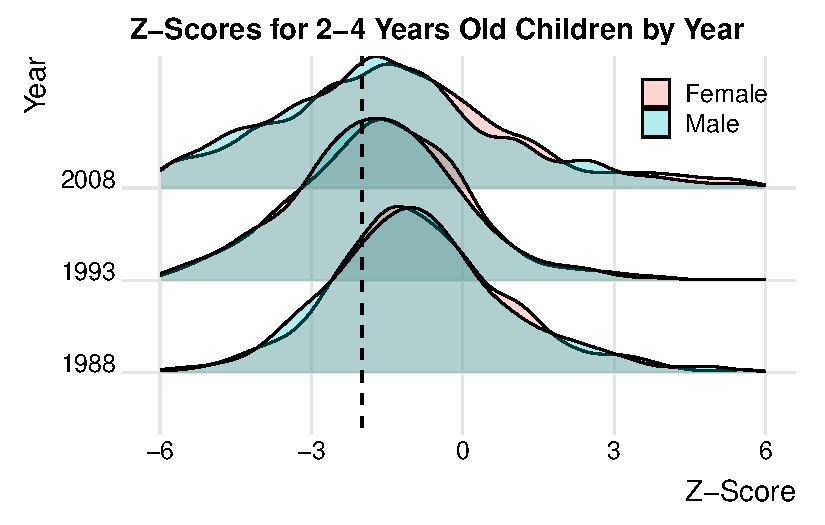
\includegraphics[keepaspectratio]{hw2_files/figure-pdf/fig-distributions_stunted-1.pdf}}

}

}

\end{figure}%

\textbf{(b) Estimate the stunting rate for 2-4 years old children over
time for boys and for girls at the national level. Decide what are
outliers, and show results both including and excluding outliers.
Comment your results, making all relevant comparisons.}

 
\begin{table}[ht]
\begin{centerbox}
\begin{threeparttable}
\captionsetup{justification=centering,singlelinecheck=off}
\caption{National stunting rates for 2-4 years old boys and girls including outliers.}
 \label{tbl-stunted_w_sex_outliers}\setlength{\tabcolsep}{0pt}
\begin{tabular}{l l l l}


\hhline{>{\huxb{0, 0, 0}{0.8}}->{\huxb{0, 0, 0}{0.8}}->{\huxb{0, 0, 0}{0.8}}->{\huxb{0, 0, 0}{0.8}}-}
\arrayrulecolor{black}

\multicolumn{1}{!{\huxvb{0, 0, 0}{0}}c!{\huxvb{0, 0, 0}{0}}}{\huxtpad{1.5pt + 1em}\centering \hspace{1.5pt}  \hspace{1.5pt}\huxbpad{1.5pt}} &
\multicolumn{1}{c!{\huxvb{0, 0, 0}{0}}}{\huxtpad{1.5pt + 1em}\centering \hspace{1.5pt} Male \hspace{1.5pt}\huxbpad{1.5pt}} &
\multicolumn{1}{c!{\huxvb{0, 0, 0}{0}}}{\huxtpad{1.5pt + 1em}\centering \hspace{1.5pt} Female \hspace{1.5pt}\huxbpad{1.5pt}} &
\multicolumn{1}{c!{\huxvb{0, 0, 0}{0}}}{\huxtpad{1.5pt + 1em}\centering \hspace{1.5pt} Diff (Male-Female) \hspace{1.5pt}\huxbpad{1.5pt}} \tabularnewline[-0.5pt]


\hhline{>{\huxb{255, 255, 255}{0.4}}->{\huxb{0, 0, 0}{0.4}}->{\huxb{0, 0, 0}{0.4}}->{\huxb{0, 0, 0}{0.4}}-}
\arrayrulecolor{black}

\multicolumn{1}{!{\huxvb{0, 0, 0}{0}}l!{\huxvb{0, 0, 0}{0}}}{\huxtpad{1.5pt + 1em}\raggedright \hspace{1.5pt} Year 1988 \hspace{1.5pt}\huxbpad{1.5pt}} &
\multicolumn{1}{r!{\huxvb{0, 0, 0}{0}}}{\huxtpad{1.5pt + 1em}\raggedleft \hspace{1.5pt} 0.271 *** \hspace{1.5pt}\huxbpad{1.5pt}} &
\multicolumn{1}{r!{\huxvb{0, 0, 0}{0}}}{\huxtpad{1.5pt + 1em}\raggedleft \hspace{1.5pt} 0.254 *** \hspace{1.5pt}\huxbpad{1.5pt}} &
\multicolumn{1}{r!{\huxvb{0, 0, 0}{0}}}{\huxtpad{1.5pt + 1em}\raggedleft \hspace{1.5pt} 0.017 \hspace{1.5pt}\huxbpad{1.5pt}} \tabularnewline[-0.5pt]


\hhline{}
\arrayrulecolor{black}

\multicolumn{1}{!{\huxvb{0, 0, 0}{0}}l!{\huxvb{0, 0, 0}{0}}}{\huxtpad{1.5pt + 1em}\raggedright \hspace{1.5pt}  \hspace{1.5pt}\huxbpad{1.5pt}} &
\multicolumn{1}{r!{\huxvb{0, 0, 0}{0}}}{\huxtpad{1.5pt + 1em}\raggedleft \hspace{1.5pt} (0.015) \hspace{1.5pt}\huxbpad{1.5pt}} &
\multicolumn{1}{r!{\huxvb{0, 0, 0}{0}}}{\huxtpad{1.5pt + 1em}\raggedleft \hspace{1.5pt} (0.016) \hspace{1.5pt}\huxbpad{1.5pt}} &
\multicolumn{1}{r!{\huxvb{0, 0, 0}{0}}}{\huxtpad{1.5pt + 1em}\raggedleft \hspace{1.5pt} (0.022) \hspace{1.5pt}\huxbpad{1.5pt}} \tabularnewline[-0.5pt]


\hhline{}
\arrayrulecolor{black}

\multicolumn{1}{!{\huxvb{0, 0, 0}{0}}l!{\huxvb{0, 0, 0}{0}}}{\huxtpad{1.5pt + 1em}\raggedright \hspace{1.5pt} Year 1993 \hspace{1.5pt}\huxbpad{1.5pt}} &
\multicolumn{1}{r!{\huxvb{0, 0, 0}{0}}}{\huxtpad{1.5pt + 1em}\raggedleft \hspace{1.5pt} 0.464 *** \hspace{1.5pt}\huxbpad{1.5pt}} &
\multicolumn{1}{r!{\huxvb{0, 0, 0}{0}}}{\huxtpad{1.5pt + 1em}\raggedleft \hspace{1.5pt} 0.413 *** \hspace{1.5pt}\huxbpad{1.5pt}} &
\multicolumn{1}{r!{\huxvb{0, 0, 0}{0}}}{\huxtpad{1.5pt + 1em}\raggedleft \hspace{1.5pt} 0.051 *** \hspace{1.5pt}\huxbpad{1.5pt}} \tabularnewline[-0.5pt]


\hhline{}
\arrayrulecolor{black}

\multicolumn{1}{!{\huxvb{0, 0, 0}{0}}l!{\huxvb{0, 0, 0}{0}}}{\huxtpad{1.5pt + 1em}\raggedright \hspace{1.5pt}  \hspace{1.5pt}\huxbpad{1.5pt}} &
\multicolumn{1}{r!{\huxvb{0, 0, 0}{0}}}{\huxtpad{1.5pt + 1em}\raggedleft \hspace{1.5pt} (0.012) \hspace{1.5pt}\huxbpad{1.5pt}} &
\multicolumn{1}{r!{\huxvb{0, 0, 0}{0}}}{\huxtpad{1.5pt + 1em}\raggedleft \hspace{1.5pt} (0.012) \hspace{1.5pt}\huxbpad{1.5pt}} &
\multicolumn{1}{r!{\huxvb{0, 0, 0}{0}}}{\huxtpad{1.5pt + 1em}\raggedleft \hspace{1.5pt} (0.017) \hspace{1.5pt}\huxbpad{1.5pt}} \tabularnewline[-0.5pt]


\hhline{}
\arrayrulecolor{black}

\multicolumn{1}{!{\huxvb{0, 0, 0}{0}}l!{\huxvb{0, 0, 0}{0}}}{\huxtpad{1.5pt + 1em}\raggedright \hspace{1.5pt} Year 2008 \hspace{1.5pt}\huxbpad{1.5pt}} &
\multicolumn{1}{r!{\huxvb{0, 0, 0}{0}}}{\huxtpad{1.5pt + 1em}\raggedleft \hspace{1.5pt} 0.479 *** \hspace{1.5pt}\huxbpad{1.5pt}} &
\multicolumn{1}{r!{\huxvb{0, 0, 0}{0}}}{\huxtpad{1.5pt + 1em}\raggedleft \hspace{1.5pt} 0.461 *** \hspace{1.5pt}\huxbpad{1.5pt}} &
\multicolumn{1}{r!{\huxvb{0, 0, 0}{0}}}{\huxtpad{1.5pt + 1em}\raggedleft \hspace{1.5pt} 0.018 \hspace{1.5pt}\huxbpad{1.5pt}} \tabularnewline[-0.5pt]


\hhline{}
\arrayrulecolor{black}

\multicolumn{1}{!{\huxvb{0, 0, 0}{0}}l!{\huxvb{0, 0, 0}{0}}}{\huxtpad{1.5pt + 1em}\raggedright \hspace{1.5pt}  \hspace{1.5pt}\huxbpad{1.5pt}} &
\multicolumn{1}{r!{\huxvb{0, 0, 0}{0}}}{\huxtpad{1.5pt + 1em}\raggedleft \hspace{1.5pt} (0.013) \hspace{1.5pt}\huxbpad{1.5pt}} &
\multicolumn{1}{r!{\huxvb{0, 0, 0}{0}}}{\huxtpad{1.5pt + 1em}\raggedleft \hspace{1.5pt} (0.014) \hspace{1.5pt}\huxbpad{1.5pt}} &
\multicolumn{1}{r!{\huxvb{0, 0, 0}{0}}}{\huxtpad{1.5pt + 1em}\raggedleft \hspace{1.5pt} (0.019) \hspace{1.5pt}\huxbpad{1.5pt}} \tabularnewline[-0.5pt]


\hhline{>{\huxb{255, 255, 255}{0.4}}->{\huxb{0, 0, 0}{0.4}}->{\huxb{0, 0, 0}{0.4}}->{\huxb{0, 0, 0}{0.4}}-}
\arrayrulecolor{black}

\multicolumn{1}{!{\huxvb{0, 0, 0}{0}}l!{\huxvb{0, 0, 0}{0}}}{\huxtpad{1.5pt + 1em}\raggedright \hspace{1.5pt} N \hspace{1.5pt}\huxbpad{1.5pt}} &
\multicolumn{1}{r!{\huxvb{0, 0, 0}{0}}}{\huxtpad{1.5pt + 1em}\raggedleft \hspace{1.5pt} 3963 \hspace{1.5pt}\huxbpad{1.5pt}} &
\multicolumn{1}{r!{\huxvb{0, 0, 0}{0}}}{\huxtpad{1.5pt + 1em}\raggedleft \hspace{1.5pt} 3771 \hspace{1.5pt}\huxbpad{1.5pt}} &
\multicolumn{1}{r!{\huxvb{0, 0, 0}{0}}}{\huxtpad{1.5pt + 1em}\raggedleft \hspace{1.5pt}  \hspace{1.5pt}\huxbpad{1.5pt}} \tabularnewline[-0.5pt]


\hhline{}
\arrayrulecolor{black}

\multicolumn{1}{!{\huxvb{0, 0, 0}{0}}l!{\huxvb{0, 0, 0}{0}}}{\huxtpad{1.5pt + 1em}\raggedright \hspace{1.5pt} R2 \hspace{1.5pt}\huxbpad{1.5pt}} &
\multicolumn{1}{r!{\huxvb{0, 0, 0}{0}}}{\huxtpad{1.5pt + 1em}\raggedleft \hspace{1.5pt} 0.438 \hspace{1.5pt}\huxbpad{1.5pt}} &
\multicolumn{1}{r!{\huxvb{0, 0, 0}{0}}}{\huxtpad{1.5pt + 1em}\raggedleft \hspace{1.5pt} 0.405 \hspace{1.5pt}\huxbpad{1.5pt}} &
\multicolumn{1}{r!{\huxvb{0, 0, 0}{0}}}{\huxtpad{1.5pt + 1em}\raggedleft \hspace{1.5pt}  \hspace{1.5pt}\huxbpad{1.5pt}} \tabularnewline[-0.5pt]


\hhline{>{\huxb{0, 0, 0}{0.8}}->{\huxb{0, 0, 0}{0.8}}->{\huxb{0, 0, 0}{0.8}}->{\huxb{0, 0, 0}{0.8}}-}
\arrayrulecolor{black}
\end{tabular}
\begin{tablenotes}[flushleft]
\item[] Significance: *** p $<$ 0.01; ** p $<$ 0.05; * p $<$ 0.1
\end{tablenotes}
\end{threeparttable}\par\end{centerbox}

\end{table}
 

 
\begin{table}[ht]
\begin{centerbox}
\begin{threeparttable}
\captionsetup{justification=centering,singlelinecheck=off}
\caption{National stunting rates for 2-4 years old boys and girls excluding outliers.}
 \label{tbl-stunted_n_sex_outliers}\setlength{\tabcolsep}{0pt}
\begin{tabular}{l l l l}


\hhline{>{\huxb{0, 0, 0}{0.8}}->{\huxb{0, 0, 0}{0.8}}->{\huxb{0, 0, 0}{0.8}}->{\huxb{0, 0, 0}{0.8}}-}
\arrayrulecolor{black}

\multicolumn{1}{!{\huxvb{0, 0, 0}{0}}c!{\huxvb{0, 0, 0}{0}}}{\huxtpad{1.5pt + 1em}\centering \hspace{1.5pt}  \hspace{1.5pt}\huxbpad{1.5pt}} &
\multicolumn{1}{c!{\huxvb{0, 0, 0}{0}}}{\huxtpad{1.5pt + 1em}\centering \hspace{1.5pt} Male \hspace{1.5pt}\huxbpad{1.5pt}} &
\multicolumn{1}{c!{\huxvb{0, 0, 0}{0}}}{\huxtpad{1.5pt + 1em}\centering \hspace{1.5pt} Female \hspace{1.5pt}\huxbpad{1.5pt}} &
\multicolumn{1}{c!{\huxvb{0, 0, 0}{0}}}{\huxtpad{1.5pt + 1em}\centering \hspace{1.5pt} Diff (Male-Female) \hspace{1.5pt}\huxbpad{1.5pt}} \tabularnewline[-0.5pt]


\hhline{>{\huxb{255, 255, 255}{0.4}}->{\huxb{0, 0, 0}{0.4}}->{\huxb{0, 0, 0}{0.4}}->{\huxb{0, 0, 0}{0.4}}-}
\arrayrulecolor{black}

\multicolumn{1}{!{\huxvb{0, 0, 0}{0}}l!{\huxvb{0, 0, 0}{0}}}{\huxtpad{1.5pt + 1em}\raggedright \hspace{1.5pt} Year 1988 \hspace{1.5pt}\huxbpad{1.5pt}} &
\multicolumn{1}{r!{\huxvb{0, 0, 0}{0}}}{\huxtpad{1.5pt + 1em}\raggedleft \hspace{1.5pt} 0.268 *** \hspace{1.5pt}\huxbpad{1.5pt}} &
\multicolumn{1}{r!{\huxvb{0, 0, 0}{0}}}{\huxtpad{1.5pt + 1em}\raggedleft \hspace{1.5pt} 0.252 *** \hspace{1.5pt}\huxbpad{1.5pt}} &
\multicolumn{1}{r!{\huxvb{0, 0, 0}{0}}}{\huxtpad{1.5pt + 1em}\raggedleft \hspace{1.5pt} 0.017 \hspace{1.5pt}\huxbpad{1.5pt}} \tabularnewline[-0.5pt]


\hhline{}
\arrayrulecolor{black}

\multicolumn{1}{!{\huxvb{0, 0, 0}{0}}l!{\huxvb{0, 0, 0}{0}}}{\huxtpad{1.5pt + 1em}\raggedright \hspace{1.5pt}  \hspace{1.5pt}\huxbpad{1.5pt}} &
\multicolumn{1}{r!{\huxvb{0, 0, 0}{0}}}{\huxtpad{1.5pt + 1em}\raggedleft \hspace{1.5pt} (0.015) \hspace{1.5pt}\huxbpad{1.5pt}} &
\multicolumn{1}{r!{\huxvb{0, 0, 0}{0}}}{\huxtpad{1.5pt + 1em}\raggedleft \hspace{1.5pt} (0.016) \hspace{1.5pt}\huxbpad{1.5pt}} &
\multicolumn{1}{r!{\huxvb{0, 0, 0}{0}}}{\huxtpad{1.5pt + 1em}\raggedleft \hspace{1.5pt} (0.022) \hspace{1.5pt}\huxbpad{1.5pt}} \tabularnewline[-0.5pt]


\hhline{}
\arrayrulecolor{black}

\multicolumn{1}{!{\huxvb{0, 0, 0}{0}}l!{\huxvb{0, 0, 0}{0}}}{\huxtpad{1.5pt + 1em}\raggedright \hspace{1.5pt} Year 1993 \hspace{1.5pt}\huxbpad{1.5pt}} &
\multicolumn{1}{r!{\huxvb{0, 0, 0}{0}}}{\huxtpad{1.5pt + 1em}\raggedleft \hspace{1.5pt} 0.456 *** \hspace{1.5pt}\huxbpad{1.5pt}} &
\multicolumn{1}{r!{\huxvb{0, 0, 0}{0}}}{\huxtpad{1.5pt + 1em}\raggedleft \hspace{1.5pt} 0.407 *** \hspace{1.5pt}\huxbpad{1.5pt}} &
\multicolumn{1}{r!{\huxvb{0, 0, 0}{0}}}{\huxtpad{1.5pt + 1em}\raggedleft \hspace{1.5pt} 0.049 *** \hspace{1.5pt}\huxbpad{1.5pt}} \tabularnewline[-0.5pt]


\hhline{}
\arrayrulecolor{black}

\multicolumn{1}{!{\huxvb{0, 0, 0}{0}}l!{\huxvb{0, 0, 0}{0}}}{\huxtpad{1.5pt + 1em}\raggedright \hspace{1.5pt}  \hspace{1.5pt}\huxbpad{1.5pt}} &
\multicolumn{1}{r!{\huxvb{0, 0, 0}{0}}}{\huxtpad{1.5pt + 1em}\raggedleft \hspace{1.5pt} (0.012) \hspace{1.5pt}\huxbpad{1.5pt}} &
\multicolumn{1}{r!{\huxvb{0, 0, 0}{0}}}{\huxtpad{1.5pt + 1em}\raggedleft \hspace{1.5pt} (0.012) \hspace{1.5pt}\huxbpad{1.5pt}} &
\multicolumn{1}{r!{\huxvb{0, 0, 0}{0}}}{\huxtpad{1.5pt + 1em}\raggedleft \hspace{1.5pt} (0.017) \hspace{1.5pt}\huxbpad{1.5pt}} \tabularnewline[-0.5pt]


\hhline{}
\arrayrulecolor{black}

\multicolumn{1}{!{\huxvb{0, 0, 0}{0}}l!{\huxvb{0, 0, 0}{0}}}{\huxtpad{1.5pt + 1em}\raggedright \hspace{1.5pt} Year 2008 \hspace{1.5pt}\huxbpad{1.5pt}} &
\multicolumn{1}{r!{\huxvb{0, 0, 0}{0}}}{\huxtpad{1.5pt + 1em}\raggedleft \hspace{1.5pt} 0.416 *** \hspace{1.5pt}\huxbpad{1.5pt}} &
\multicolumn{1}{r!{\huxvb{0, 0, 0}{0}}}{\huxtpad{1.5pt + 1em}\raggedleft \hspace{1.5pt} 0.397 *** \hspace{1.5pt}\huxbpad{1.5pt}} &
\multicolumn{1}{r!{\huxvb{0, 0, 0}{0}}}{\huxtpad{1.5pt + 1em}\raggedleft \hspace{1.5pt} 0.019 \hspace{1.5pt}\huxbpad{1.5pt}} \tabularnewline[-0.5pt]


\hhline{}
\arrayrulecolor{black}

\multicolumn{1}{!{\huxvb{0, 0, 0}{0}}l!{\huxvb{0, 0, 0}{0}}}{\huxtpad{1.5pt + 1em}\raggedright \hspace{1.5pt}  \hspace{1.5pt}\huxbpad{1.5pt}} &
\multicolumn{1}{r!{\huxvb{0, 0, 0}{0}}}{\huxtpad{1.5pt + 1em}\raggedleft \hspace{1.5pt} (0.015) \hspace{1.5pt}\huxbpad{1.5pt}} &
\multicolumn{1}{r!{\huxvb{0, 0, 0}{0}}}{\huxtpad{1.5pt + 1em}\raggedleft \hspace{1.5pt} (0.015) \hspace{1.5pt}\huxbpad{1.5pt}} &
\multicolumn{1}{r!{\huxvb{0, 0, 0}{0}}}{\huxtpad{1.5pt + 1em}\raggedleft \hspace{1.5pt} (0.021) \hspace{1.5pt}\huxbpad{1.5pt}} \tabularnewline[-0.5pt]


\hhline{>{\huxb{255, 255, 255}{0.4}}->{\huxb{0, 0, 0}{0.4}}->{\huxb{0, 0, 0}{0.4}}->{\huxb{0, 0, 0}{0.4}}-}
\arrayrulecolor{black}

\multicolumn{1}{!{\huxvb{0, 0, 0}{0}}l!{\huxvb{0, 0, 0}{0}}}{\huxtpad{1.5pt + 1em}\raggedright \hspace{1.5pt} N \hspace{1.5pt}\huxbpad{1.5pt}} &
\multicolumn{1}{r!{\huxvb{0, 0, 0}{0}}}{\huxtpad{1.5pt + 1em}\raggedleft \hspace{1.5pt} 3627 \hspace{1.5pt}\huxbpad{1.5pt}} &
\multicolumn{1}{r!{\huxvb{0, 0, 0}{0}}}{\huxtpad{1.5pt + 1em}\raggedleft \hspace{1.5pt} 3484 \hspace{1.5pt}\huxbpad{1.5pt}} &
\multicolumn{1}{r!{\huxvb{0, 0, 0}{0}}}{\huxtpad{1.5pt + 1em}\raggedleft \hspace{1.5pt}  \hspace{1.5pt}\huxbpad{1.5pt}} \tabularnewline[-0.5pt]


\hhline{}
\arrayrulecolor{black}

\multicolumn{1}{!{\huxvb{0, 0, 0}{0}}l!{\huxvb{0, 0, 0}{0}}}{\huxtpad{1.5pt + 1em}\raggedright \hspace{1.5pt} R2 \hspace{1.5pt}\huxbpad{1.5pt}} &
\multicolumn{1}{r!{\huxvb{0, 0, 0}{0}}}{\huxtpad{1.5pt + 1em}\raggedleft \hspace{1.5pt} 0.409 \hspace{1.5pt}\huxbpad{1.5pt}} &
\multicolumn{1}{r!{\huxvb{0, 0, 0}{0}}}{\huxtpad{1.5pt + 1em}\raggedleft \hspace{1.5pt} 0.375 \hspace{1.5pt}\huxbpad{1.5pt}} &
\multicolumn{1}{r!{\huxvb{0, 0, 0}{0}}}{\huxtpad{1.5pt + 1em}\raggedleft \hspace{1.5pt}  \hspace{1.5pt}\huxbpad{1.5pt}} \tabularnewline[-0.5pt]


\hhline{>{\huxb{0, 0, 0}{0.8}}->{\huxb{0, 0, 0}{0.8}}->{\huxb{0, 0, 0}{0.8}}->{\huxb{0, 0, 0}{0.8}}-}
\arrayrulecolor{black}
\end{tabular}
\begin{tablenotes}[flushleft]
\item[] Significance: *** p $<$ 0.01; ** p $<$ 0.05; * p $<$ 0.1
\end{tablenotes}
\end{threeparttable}\par\end{centerbox}

\end{table}
 

\subsection{4. Height Stature and poverty (2
points)}\label{height-stature-and-poverty-2-points}

\textbf{Here, one would like to study how the gradient of the number of
stunted children aged 2-4 years, and of household consumption per
capita, as well as the relationship between the two, have changed over
time.} \textbf{Find a graphical or regression framework to represent
this (many options are possible). Comment on your results and their
limits.}

{[}Your answer here{]}

\section{3 A meaningful table (6 pts)}\label{a-meaningful-table-6-pts}

\textbf{Construct a small statistical table showing a meaningful and
policy relevant social fact about migration in the world. You may focus,
or not, on a given region or country of origin, or on a particular
subgroup of the population (children, etc.) A combination of
originality, policy relevance and statistical accuracy will be very much
appreciated. The table should fit in the top half of a page. It should
have the attributes of a proper research-paper table: title, notes, etc.
Table notes should indicate the source of data, the coverage (countries
and population), the definition and units of variables and any other
kind of information that is needed to read and understand the table. The
bottom half of the page should be dedicated to a brief text, commenting
upon the social fact that the table reveals.}{[}cite: 31{]}

{[}Your table and text here{]}

\section{Appendix: R Script}\label{appendix-r-script}

\emph{Please do not show your R script before every question, but put
your entire R script at the end of the homework.}




\end{document}
